\chapter{Background}
This chapter describes the hardware and software tools used in the project.

\section{Hardware}
\subsection{Particle Photon}
The Particle Photon is a tiny board (1.44mm $\times$ 0.8mm $\times$ 0.17mm in our configuration, weighing in at 5 grams) specifically designed for IoT\footnote{Internet of Things: a system of typically embedded devices that connects to the Internet and to each other, without requiring human-to-human or human-to-computer interaction \cite{WikipediaIoT}. There's no baseline or standard definition, which is why IEEE is still asking for suggestions to the community to provide it \cite{IEEEIoT}.} projects \cite{ParticlePhoton}, based on a relatively powerful but power efficient microcontroller of the STM32 ARM Cortex M3 family, with integrated Wi-Fi and the ability to interface itself with cloud services offered by Particle.\\
Unfortunately, the integrated Wi-Fi module was not powerful enough to ensure a reliable connection in the tested scenarios, causing frequent disconnections. An Airgain's IPEX antenna, easily pluggable to the Photon through a U.FL connector, has allowed to achieve a more stable connection.
The code deployment can be performed easily through a web-based IDE, that compiles and flashes the code to the selected device OTA (Over-The-Air). It is also possible to control the real-time device's status through a web-based too console, that allows to flash the firmware to a specific version (downgrades are trickier than upgrades, especially OTA), and displays graphs for data such Wi-Fi's signal strength and quality, round trip time and memory usage.

\begin{center}
	\begin{figure}[ht!]
		\makebox[\textwidth]{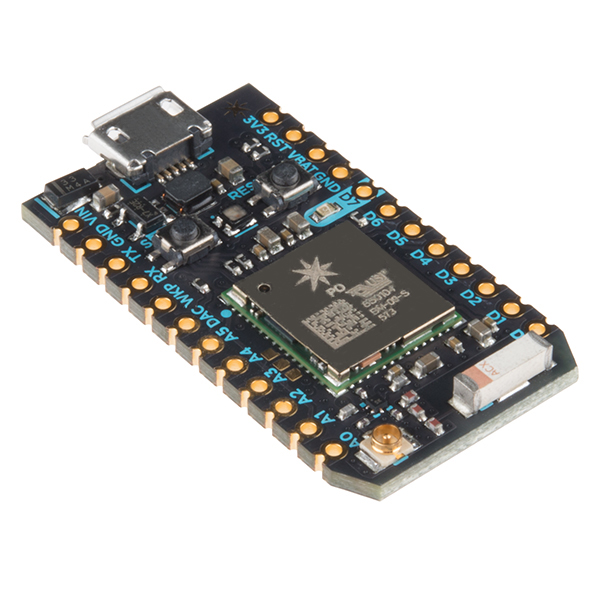
\includegraphics[width=0.3\paperwidth]{img/photon.jpg}}
		\caption{Particle Photon \cite{Photon}.}
	\end{figure}
\end{center}

\subsection{Sensors}
The SparkFun's sensor stick used in the project is a 9DoF (Degrees of Freedom) MARG (Magnetic, Angular Rate and Gravity) sensor. Its inertial module is the STMicroelectronics's LSM9DS1 integrated circuit, that features a digital linear acceleration sensor a digital angular rate sensor and a digital magnetic sensor: each one can make measurements from $x$, $y$ and $z$ axes, and that's where the 9 degrees of freedom came from. The stick has been connected to the Photon through the I$^2$C serial bus interface. Its compact size and power efficiency make it ideal for embedded systems \cite{SensorDatasheet}.
\begin{center}
	\begin{figure}[ht!]
		\makebox[\textwidth]{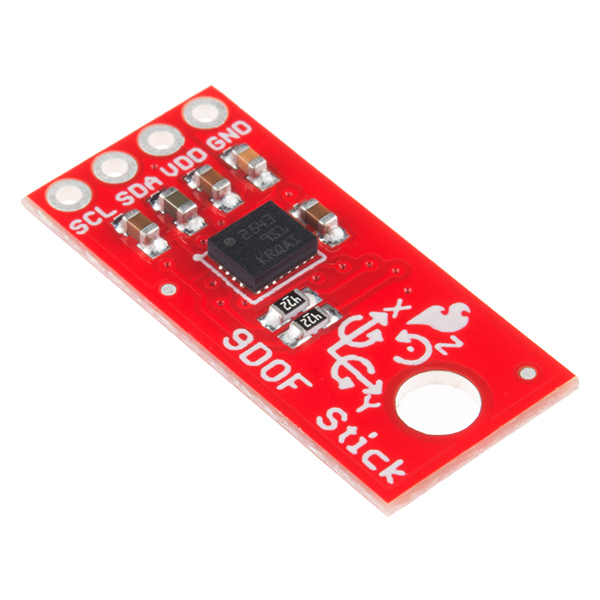
\includegraphics[width=0.3\paperwidth]{img/imu.jpg}}
		\caption{SparkFun Sensor Stick \cite{IMU}.}
	\end{figure}
\end{center}

\section{Software}
The MoVEAS software can be split in two major components: the client side part, to collect and filter sensors' data, and the server side one, to receive and manage that data.

\subsection{Node.js}
Node.js is an open-source asynchronous event-driven JavaScript runtime environment that executes code outside of a browser, built on Google Chrome's V8 JavaScript engine \cite{Node.js}.\\
To put it simply, a synchronous execution environment needs to wait to one task to finish before moving to another; asynchronous execution, on the contrary, allows to move to another task before the previous one finishes. In a network context (I/O bound), for a single-threaded software (like Node.js) a asynchronous (non-blocking) I/O (input/output) method allows to register the clients' requests, wait for until the reply is available, and then call the related callback, allowing faster replies to the clients, compared to synchronous (blocking) I/O.

\subsection{Express.js}
Express.js, or simply Express, is a minimalist, open-source web framework for Node.js, designed for building web applications and APIs \cite{Express.js}. Its main feature is the routing mechanism: it allows to specify a callback function called when the application receives a request to the specified route and HTTP method. For example, using an Express \texttt{app} object, \texttt{app.get()} would handle GET requests, \texttt{app.post()} would handle POST ones, and so on.

\subsection{Three.js}
\dots

\subsection{Pug}
\dots

\subsection{MQTT}
\dots

\subsection{MongoDB}
\dots

\subsection{TensorFlow}
\dots
